\documentclass{report}
\usepackage {mathtext}
\usepackage{amsmath}
\usepackage [russian] {babel}
\usepackage{caption}
\usepackage{subcaption}
\captionsetup[table]{position=t,justification=raggedleft,slc=off}
\setlength{\abovecaptionskip}{1pt}
\usepackage {geometry}
\usepackage {amssymb}
\usepackage{graphicx}
\geometry{margin=1in}
\title{Лабораторная работа №1.1.4. \\ Изучение статистических закономерностей на примере измерения фона космического излучения}
\author{Павел Рудачихин \\ Б04-507}
\date{11.09.2025}
\begin {document}
	\maketitle{}
	\section* {Аннотация} 
	
	\hspace{4mm} В работе измеряется радиационный фон космического излучения, на примере чего исследуются статистические методы и закономерности.
	
	\textbf{Цель работы:} на примере статистики регистрации фоновых космических частиц изучить статистические закономерности однородного во времени случайного процесса; проверить возможность описания исследуемого процесса статистическими законами Пуассона и Гаусса; измерить среднее число регистрируемых космических лучей в секунду и определить погрешность результата.

	\textbf{В работе используются:} счётчик Гейгера-Мюллера, компьютер с интерфейсом для связи со счётчиком, расчётная программа.
	
	\textbf{Методы:} статистическая обработка числовых данных программными средствами.
	
		
	\section* {Теоретические сведения}
	
	\subsection*{Счётчик Гейгера-Мюллера}
	
	
	\hspace{4mm} В данной работе для регистрации космического излучения используется счётчик Гейгера—Мюллера. Счётчик представляет собой наполненный газом металлический цилиндр с двумя электродами (корпус - катод, тонкий проводник на оси - анод). На счётчик подаётся высокое напряжение (400 В). Радиоактивное излучение ионизует молекулы газа и выбивает электроны из катода. Образовавшиеся электроны, двигаясь в сильном электрическом  поле,  соударяются  с  молекулами газа, выбивая из них новые — вторичные электроны. В результате образуется лавина электронов, и через счётчик протекает кратковременный импульс тока. Он регистрируется электрической цепью установки, оцифровывается платой аналогово-цифрового преобразователя, и информация о нём через USB-интерфейс передаётся на компьютер.
	
	Число зарегистрированных частиц за некоторое время t при фиксированном  положении  конкретного  счётчика зависит от средней интенсивности ионизирующего излучения и времени t. 
	
	\subsection*{Понятия математической статистики}
	
	\hspace{4mm} Интенсивность космического излучения - \textit{флуктуирующая} (имеющая случайные колебания) величина. Поэтому наибольшее влияние оказывают \textit{статистические} погрешности, остальными можно пренебречь.
	
	Результат измерений - это некоторая \textit{выборка} N значений $x$. Введём некоторые понятия математической статистики, применяемые в данной работе.
	
	\textit{Закон больших чисел} утверждает стремление \textit{выборочного среднего}:
	
	\begin{equation}
		\langle x \rangle = \frac{1}{N} \sum_{i=1}^{N}x_{i}
	\end{equation}
	
	к \textit{математическому ожиданию} ($Ex$) случайной величины с ростом числа измерений:
	
	\begin{equation}
		Ex = \lim_{N \rightarrow \infty} \langle x \rangle 
	\end{equation}
	
	На практике число измерений N конечно. Поэтому принимают:
	
	\begin{equation}
		Ex \approx \langle x \rangle 
	\end{equation}
	
	Кроме среднего значения важно знать, насколько сильно меняются (флуктуируют) полученные значения. Количественной мерой флуктуаций является\textit{ среднеквадратичное (стандартное) отклонение} $\sigma_x$:
	
	\begin{equation}
		\sigma_x = \sqrt{D},
	\end{equation}
	
	где $D$ - \textit{дисперсия}:
	
	\begin{equation}
		D = \frac{1}{N} \sum_{i=1}^{N} (x_{i} - \langle x \rangle)^{2}
	\end{equation}
	
	Аналогично матожиданию дисперсия (а значит, и стандартное отклонение) стремится к истинному значению при большом числе измерений.
	
	Результатом обработки выборки станет набор \textit{частот} (долей случаев) всех значений по выборке. Ожидается, что полученное \textit{распределение} соответствует распределению Пуассона.
	
	\subsection*{Распределение Пуассона}
	
	Случайный процесс является пуассоновским, если случайные события
	\begin{itemize}
		\item однородны по времени,
		\item независимы.
	\end{itemize}
	
	Распределение Пуассона имеет вид:
	
	\begin{equation}
		P(x) = \frac{(a)^{x}}{x!} e^{-a},
	\end{equation}
	
	где $P(x)$ - вероятность того, что значение случайной величины равно числу $x$, $a$ - параметр распределения. Для пуассоновского процесса этот параметр равен матожиданию и дисперсии случайной величины. По формулам (3) и (4) на практике имеем:
	
	\begin{equation}
		\sigma_{x} \approx \sqrt{\langle x \rangle}
	\end{equation}
	
	При больших значениях $\langle x \rangle$ (на практике $\gtrapprox 10$) распределение Пуассона переходит в \textit{нормальное распределение} (Гаусса).
	
	\subsection*{Распределение Гаусса}
	
	Нормальное распределение задано формулой:
	
	\begin{equation}
		P(x) = \frac{e^\frac{-(x-Ex)^{2}}{2\sigma^{2}}}{\sigma \sqrt{2\pi}}
	\end{equation}
	
	Для распределения Гаусса известны следующие вероятности того, что значение попадёт в определённый интервал:
	
	\begin{table}[h]
		\centering
		\captionbox{Свойство распределения Гаусса}{
		\begin{tabular}{|c|c|}
			\hline
			Интервал & Вероятность \\
			\hline
			$\langle x \rangle \pm \sigma$ & 68\%  \\
			\hline
			$\langle x \rangle \pm 2 \sigma$ & 95\%  \\
			\hline
			$\langle x \rangle \pm 3 \sigma$ & 99,7\%  \\
			\hline
		\end{tabular}}
	\end{table}
	
	\subsection*{Погрешность среднего}
	
	\hspace{4mm} Так как количество измерений ограничено, матожидание случайной величины оценивается через выборочное среднее с некоторой точностью. Погрешность среднего определена следующим образом:
	
	\begin{equation}
		\sigma_{\langle x \rangle} = \frac{\sigma_{x}}{\sqrt{N}}
	\end{equation}
	
	Истинное среднее значение (матожидание случайной величины) лежит в интервале:
	
	\begin{equation}
		\langle x \rangle \pm \sigma_{\langle x \rangle}
	\end{equation}
	
	Измерения произведены в автоматическом режиме с помощью программных средств, поэтому вместо методики измерений рассмотрим методику обработки данных.
	
	\section*{Методика обработки результатов измерений}
	
	\hspace{4mm} Кроме среднего и дисперсии важно также иметь представление о частоте значений x. Для этого построим \textit{гистограмму}: отложим по оси абсцисс количество частиц $x$, по оси ординат - долю случаев $w(x)$, в которых было зафиксировано данное количество частиц, по полученным точкам построим прямоугольники, высота которых - значение $w(x)$, ширина - интервал значений $x$ (в нашем случае ширина единичная). 
	
	Гистограммы построены с помощью компьютерной программы Microsoft Excel, данные подготовлены (разбиты на интервалы группировки и подсчитаны частоты) с помощью компьютерной программы, написанной на языке Python специально для этих целей. Исходные коды представлены на рис. 1.
	
	\begin{figure} [!h]
		\centering
		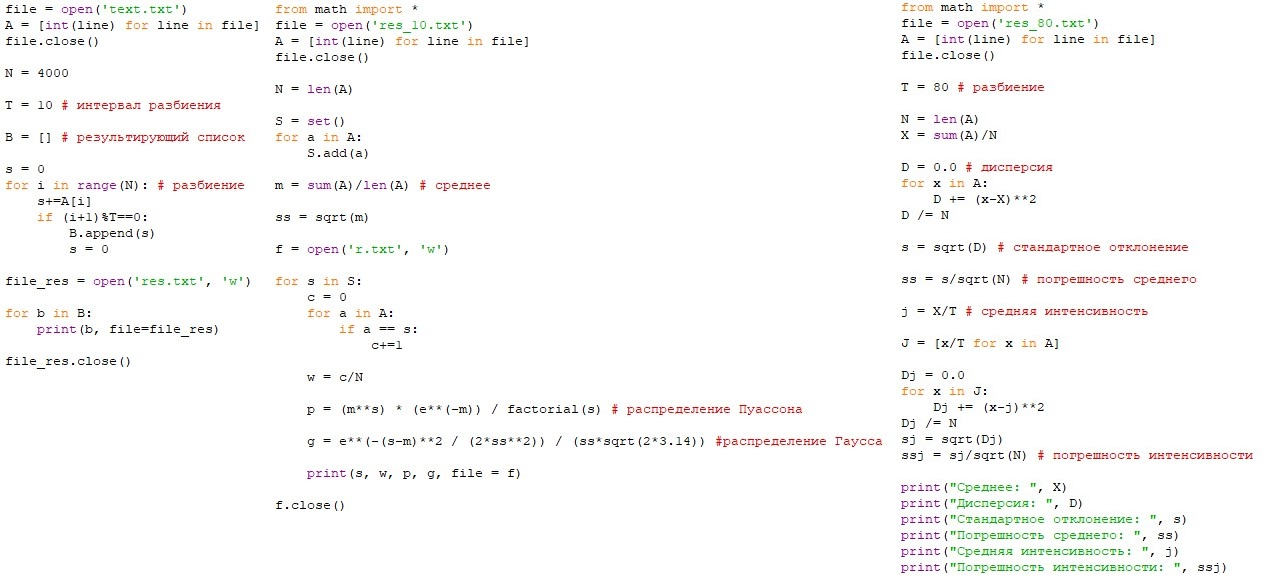
\includegraphics[width=1\linewidth]{code.jpg}
		\caption{Программы разбиения, распределения и обработки данных}
		\label{fig:code1}
	\end{figure}
	
	\section*{Работа с симуляцией}
	
	\hspace{4mm} Во время сбора экспериментальных данных было выполнено демонстрационное задание по работе с симуляцией эксперимента на основе генератора псевдослучайных чисел. В результате наблюдений при увеличении N выявлены следующие качественные зависимости:
	
	\begin{itemize}
		\item среднее число зарегистрированных частиц $\langle x \rangle$ вначале хаотически меняется в больших пределах, затем стабилизуется около значения $1,0$ (рис.2);
		\item среднеквадратичное отклонение $\sigma_{x}$ ведёт себя аналогично (рис. 3);
		\item свойство распределения Пуассона (7) хорошо выполняется при больших N;
		\item погрешность среднего $\sigma_{\langle x \rangle}$ уменьшается, в двойном логарифмическом масштабе оно почти линейно убывает (рис. 4), что говорит о том, что $\sigma_{\langle x \rangle} \rightarrow 0$;
		\item доля значений, больших 1, падает, максимум гистограммы смещается вправо; гистограмма хорошо совпадает с графиком распределения Пуассона, а с распределением Гаусса не соотносится на больших значениях.
	\end{itemize}
	
	\begin{figure}[!h]
		\centering
		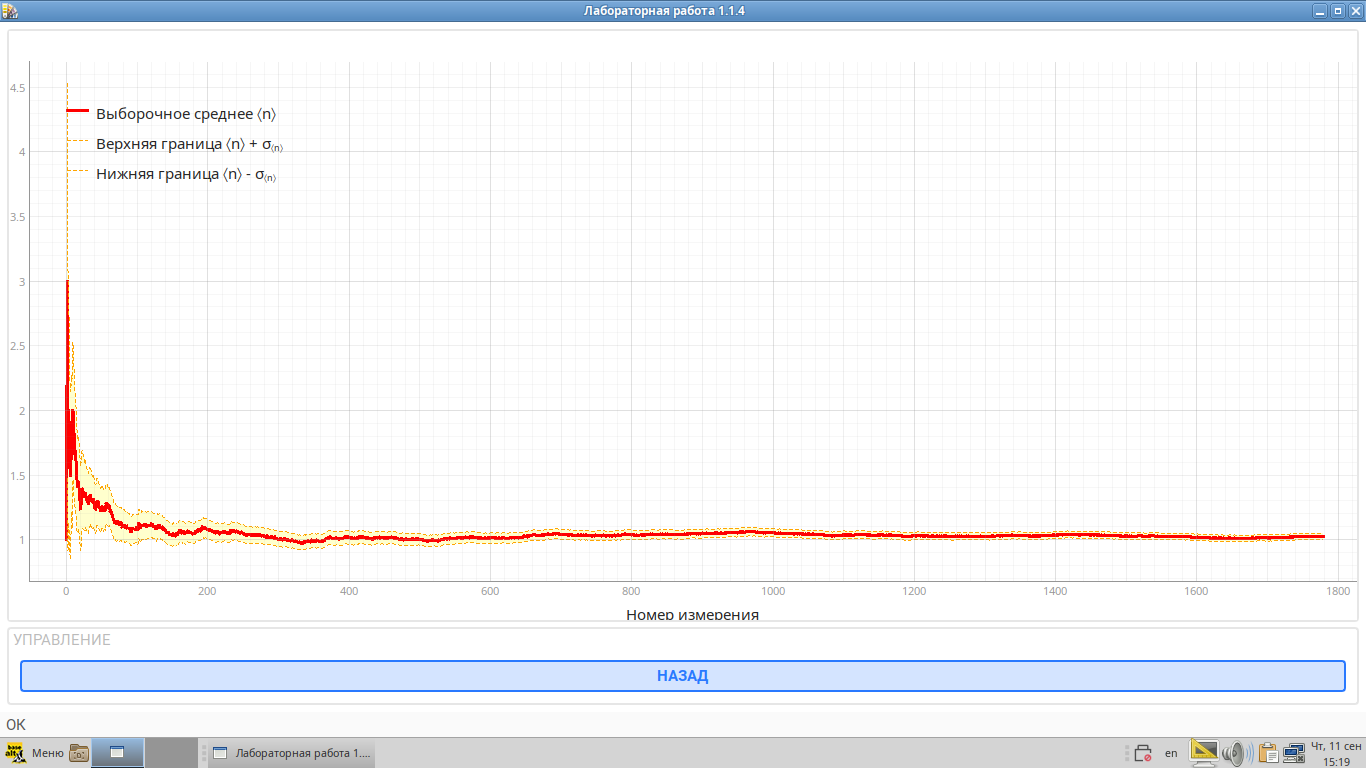
\includegraphics[width=0.6\linewidth]{pic3.png}
		\caption{Среднее число зарегистрированных частиц}
		\label{fig:1}
	\end{figure}
	\begin{figure}[!h]
		\centering
		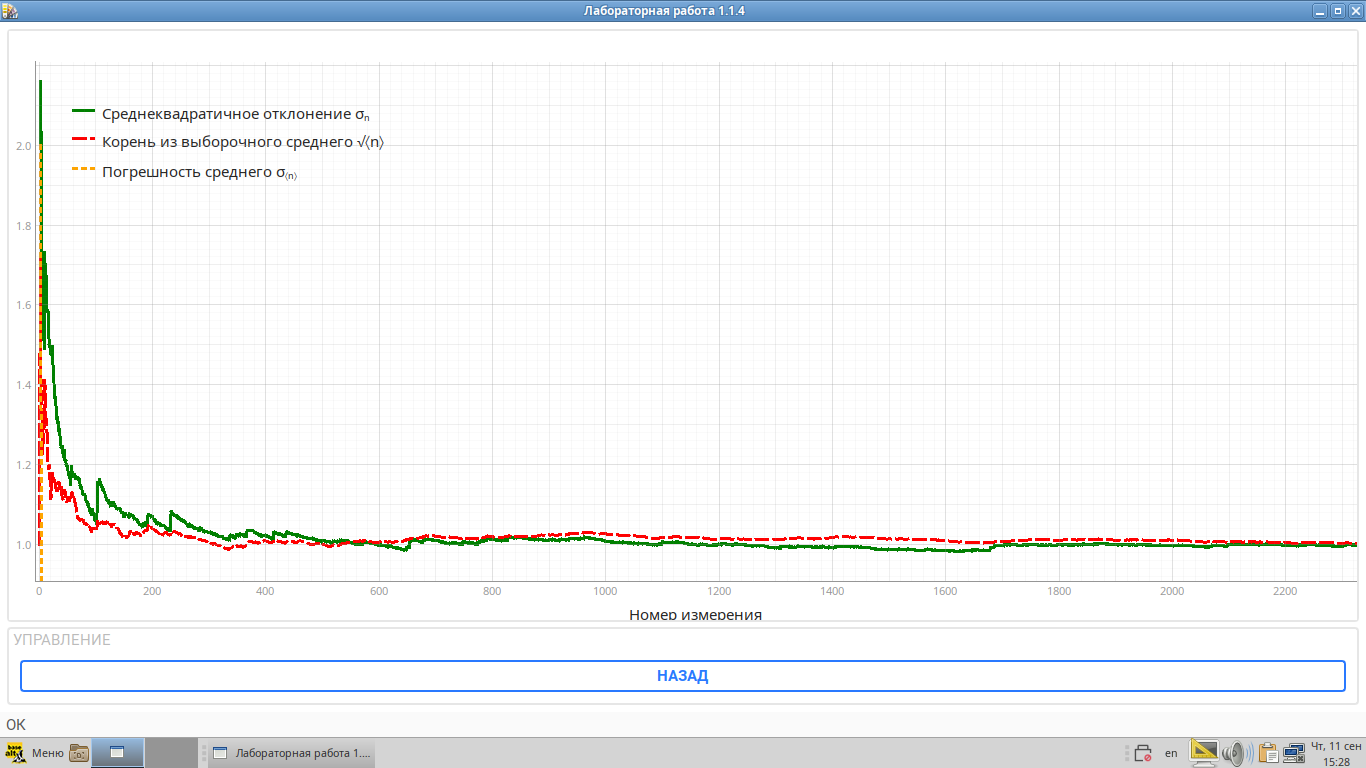
\includegraphics[width=0.6\linewidth]{pic1.png}
		\caption{Среднее значение и среднеквадратичное отклонение}
		\label{fig:2}
	\end{figure}
	\begin{figure}[!h]
		\centering
		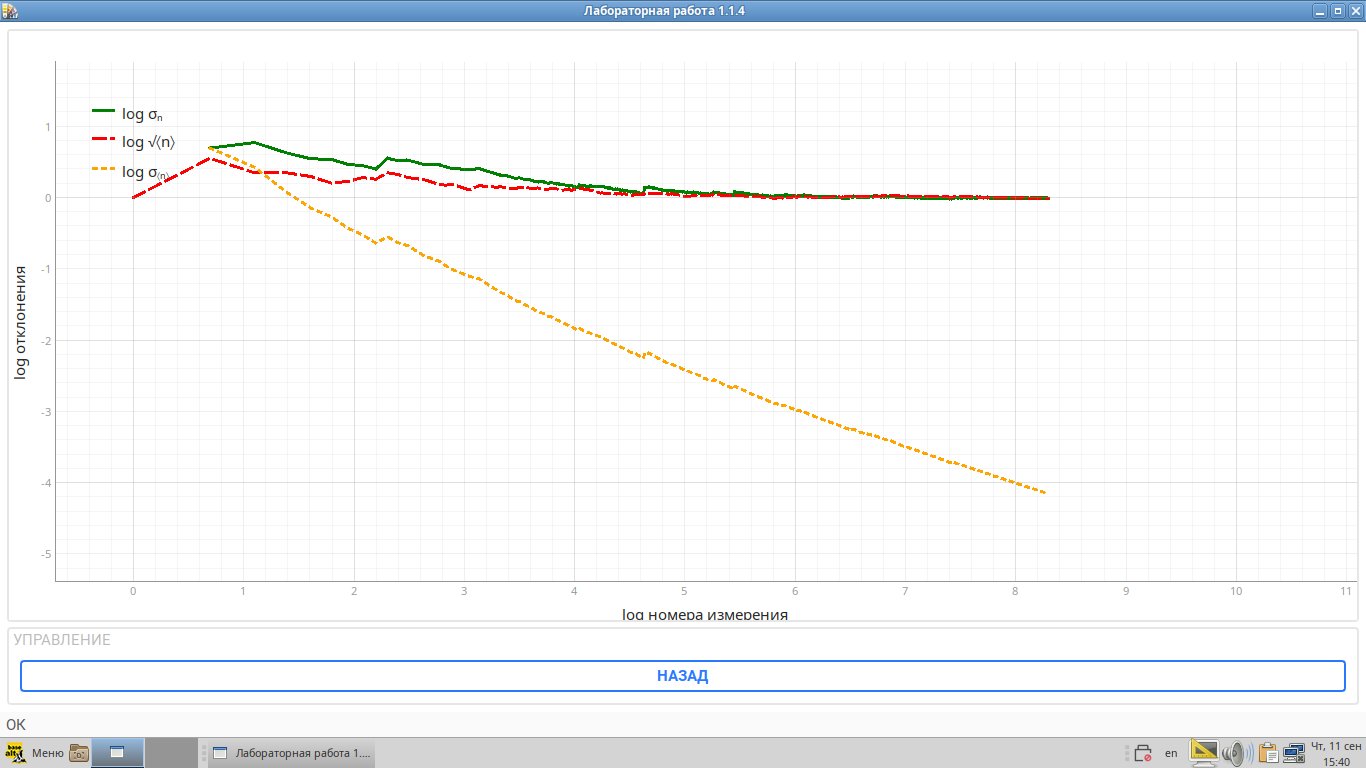
\includegraphics[width=0.6\linewidth]{pic2.png}
		\caption{Погрешность среднего в двойном логарифмическом масштабе}
		\label{fig:3}
	\end{figure}
	
	Результаты симуляции были сгруппированы с интервалами 10 с, 20 с и 80 с (рис. 5). При разбиении по 10 с гистограмма близка к распределению Гаусса. При интервалах 20 с и 80 с график не соотносится с распределениями Гаусса и Пуассона.
	 
	\begin{figure}[!h]
		\begin{subfigure}{0.5\linewidth}
			\centering
			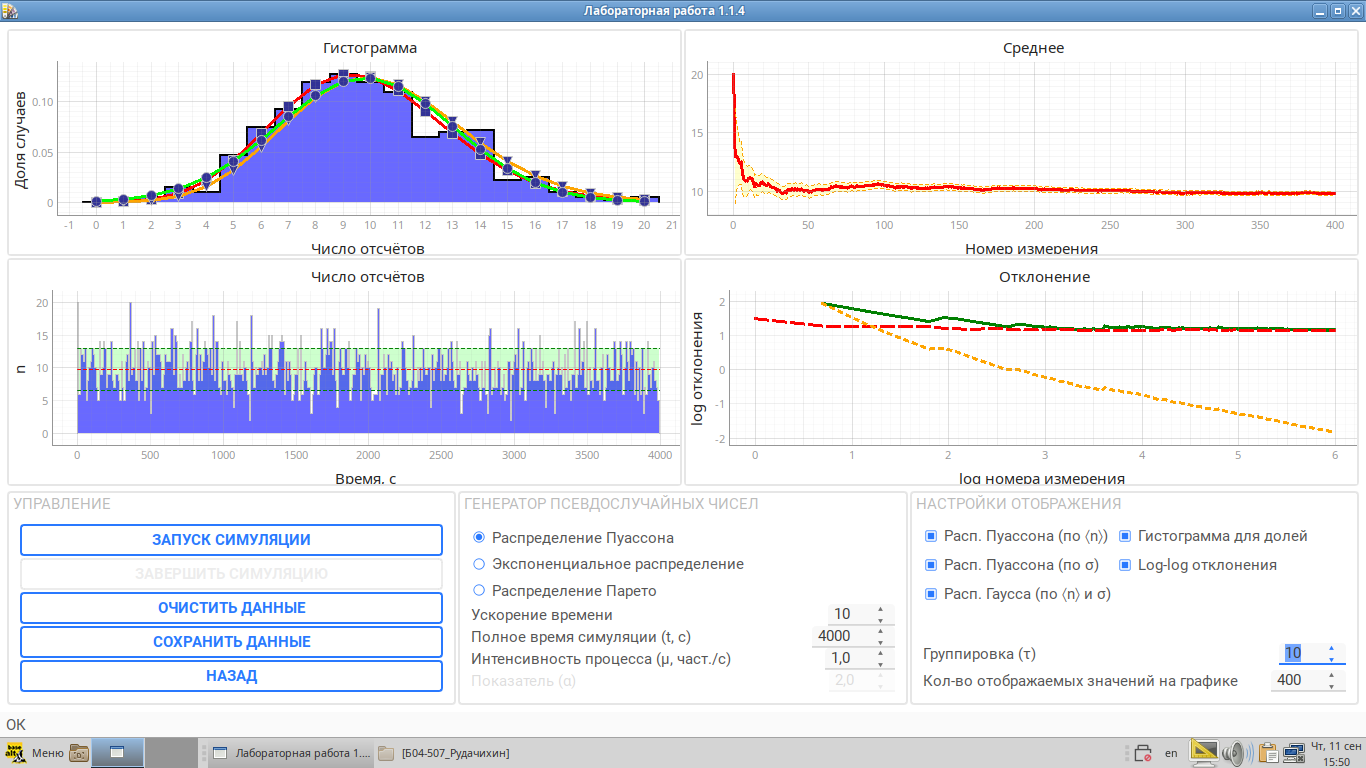
\includegraphics[width=0.9\linewidth]{pic10.png} 
			\caption{Интервал группировки 10 с}
			\label{fig:subim11}
		\end{subfigure}
		\begin{subfigure}{0.5\linewidth}
			\centering
			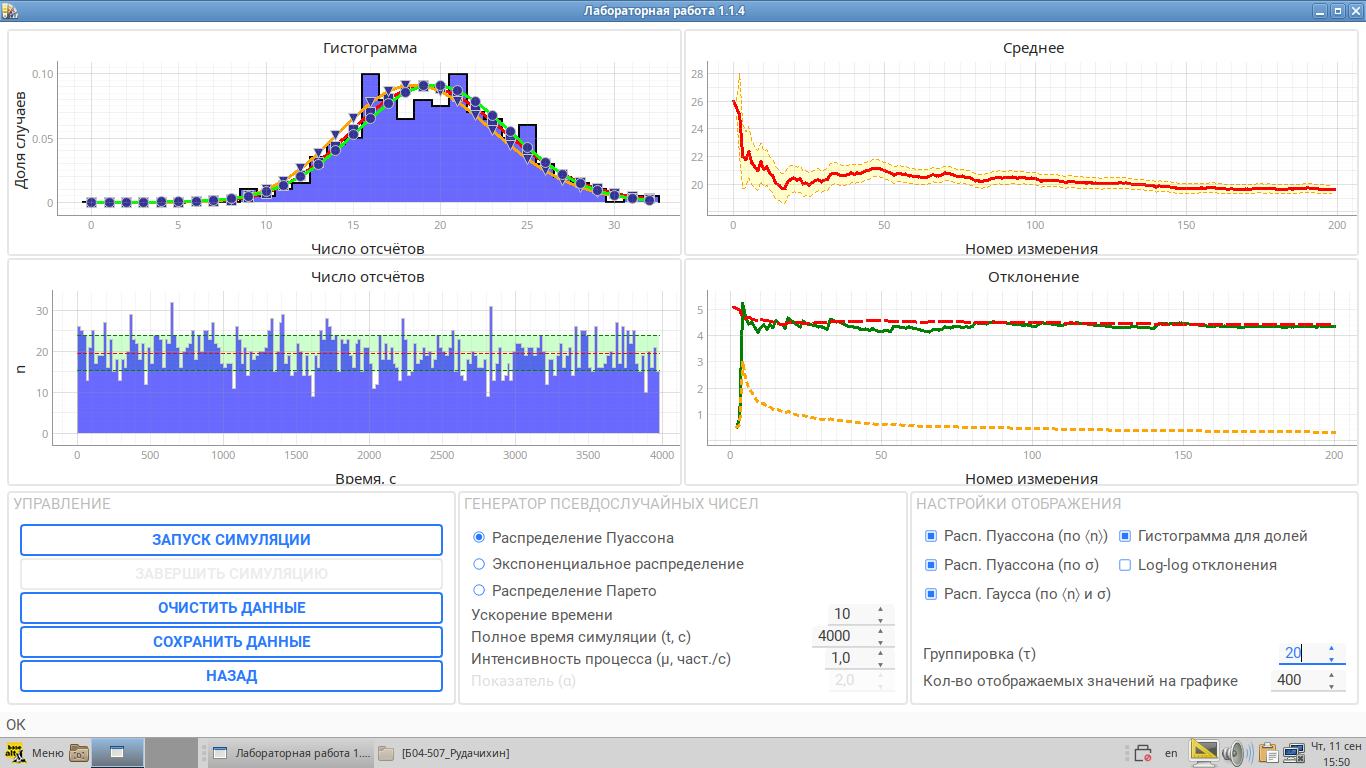
\includegraphics[width=0.9\linewidth]{pic20.png}
			\caption{Интервал группировки 20 с}
			\label{fig:subim12}
		\end{subfigure}
		\begin{subfigure}{0.5\linewidth}
			\centering
			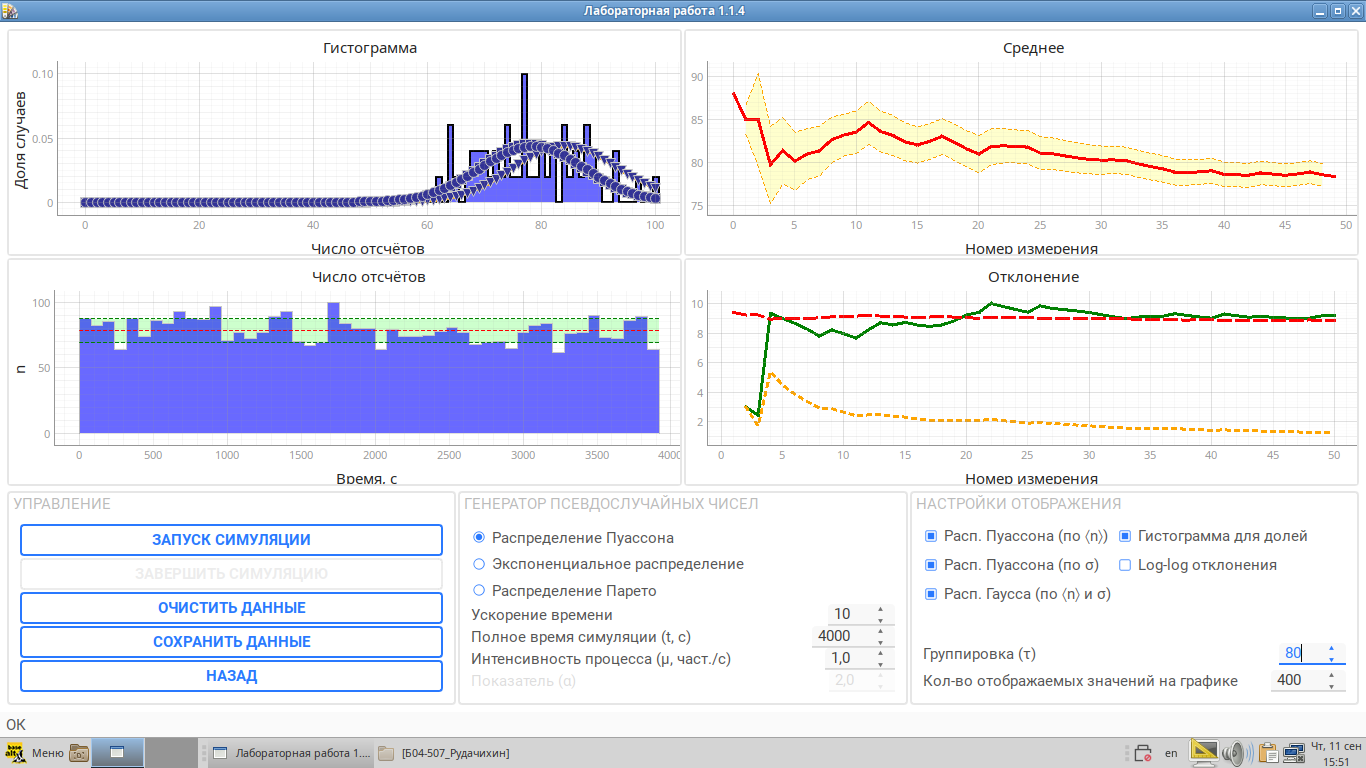
\includegraphics[width=0.9\linewidth]{pic80.png}
			\caption{Интервал группировки 80 с}
			\label{fig:subim13}
		\end{subfigure}
		\caption{Изменение интервала группировки}
		\label{fig:image12}
	\end{figure}
	
	Симуляция позволяет менять параметр $\mu$ - среднюю интенсивность частиц. Получены распределения для значений 0,1 , 10 и 100 (рис. 6). При увеличении числа измерений при единичном интервале группировки среднее значение приближается к средней интенсивности: $\langle x \rangle \approx \mu$.
	
	\begin{figure}[!h]
		\begin{subfigure}{0.5\linewidth}
			\centering
			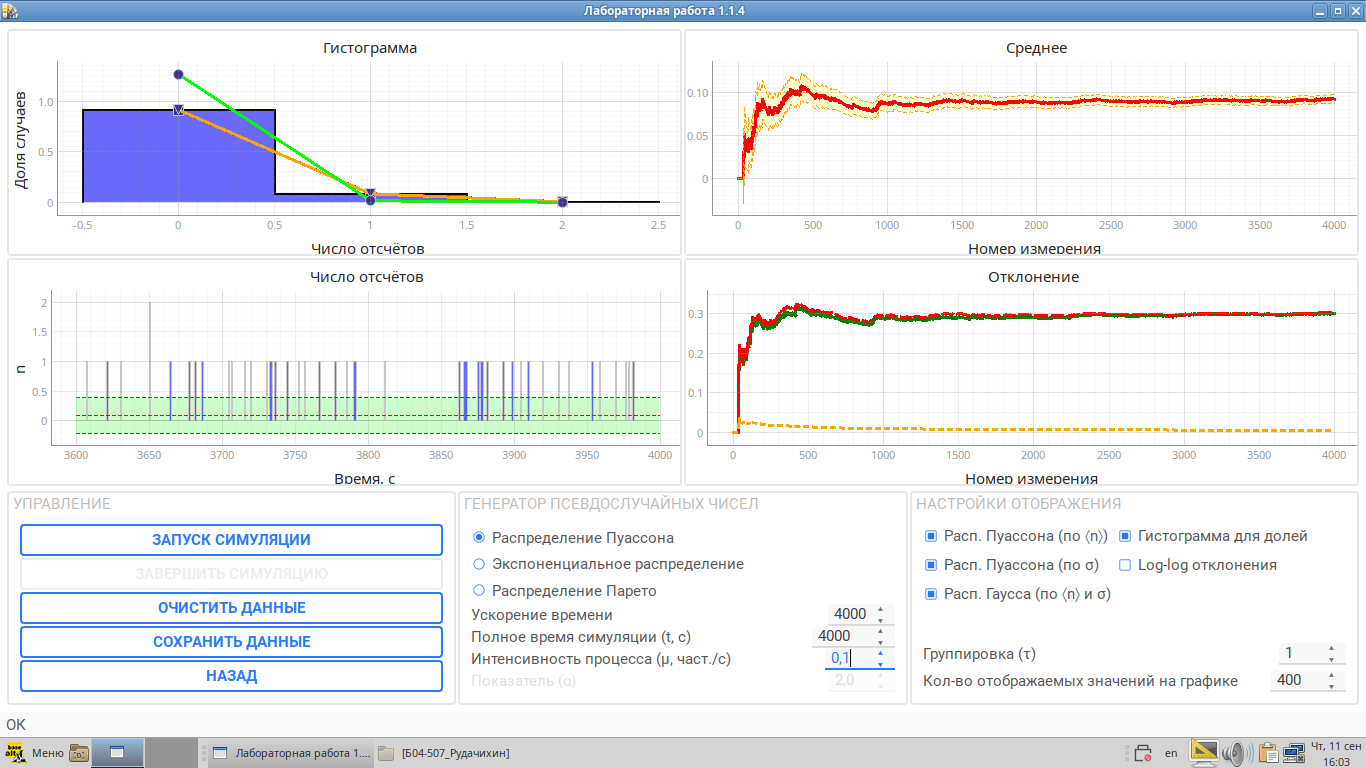
\includegraphics[width=0.9\linewidth]{pic01.png} 
			\caption{Средняя интенсивность 0,1}
			\label{fig:subim1}
		\end{subfigure}
		\begin{subfigure}{0.5\linewidth}
			\centering
			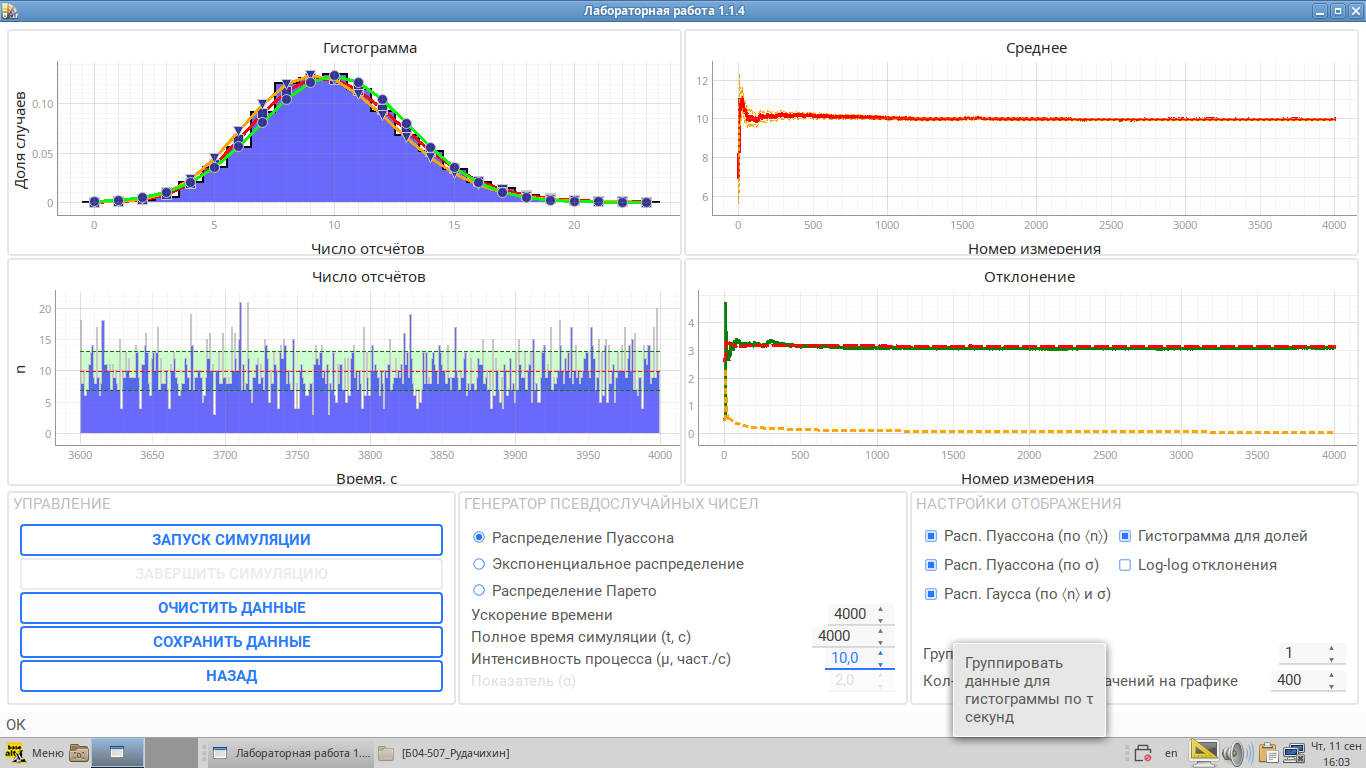
\includegraphics[width=0.9\linewidth]{pic010.png}
			\caption{Средняя интенсивность 10}
			\label{fig:subim2}
		\end{subfigure}
		\begin{subfigure}{0.5\linewidth}
			\centering
			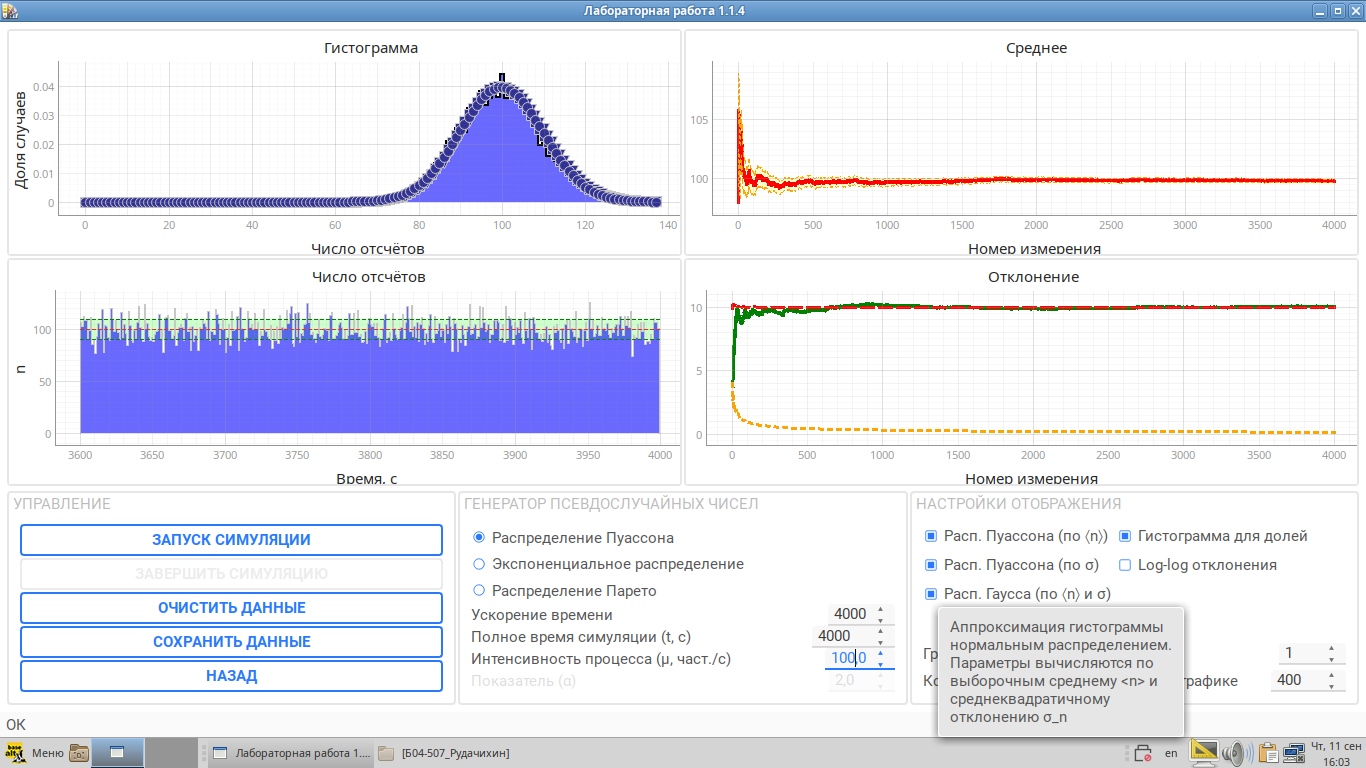
\includegraphics[width=0.9\linewidth]{pic0100.png}
			\caption{Средняя интенсивность 100}
			\label{fig:subim3}
		\end{subfigure}
		\caption{Изменение средней интенсивности}
		\label{fig:image2}
	\end{figure}
	
	В демонстрационной программе также реализованы симуляции других распределений: экспоненциального и Парето. Определено, что экспоненциальное распределение сходится с распределением Пуассона только при единичной интенсивности. С ростом интенсивности корень из среднего и среднеквадратичное отклонение не равны, гистограмма отлична от графиков теоретических распределений (рис. 7).
	
	Гистограмма распределения Парето не соотносится с распределением Гаусса, в частности из-за длинного <<хвоста>> - больших значений с низкой долей случаев. Среднее значение меняется немонотонно - <<скачками>>, т.е. не сходится к матожиданию (рис. 8). Значит, для распределения Парето не выполняется закон больших чисел.
	
	\begin{figure}[h]
		\begin{subfigure}{0.5\linewidth}
			\centering
			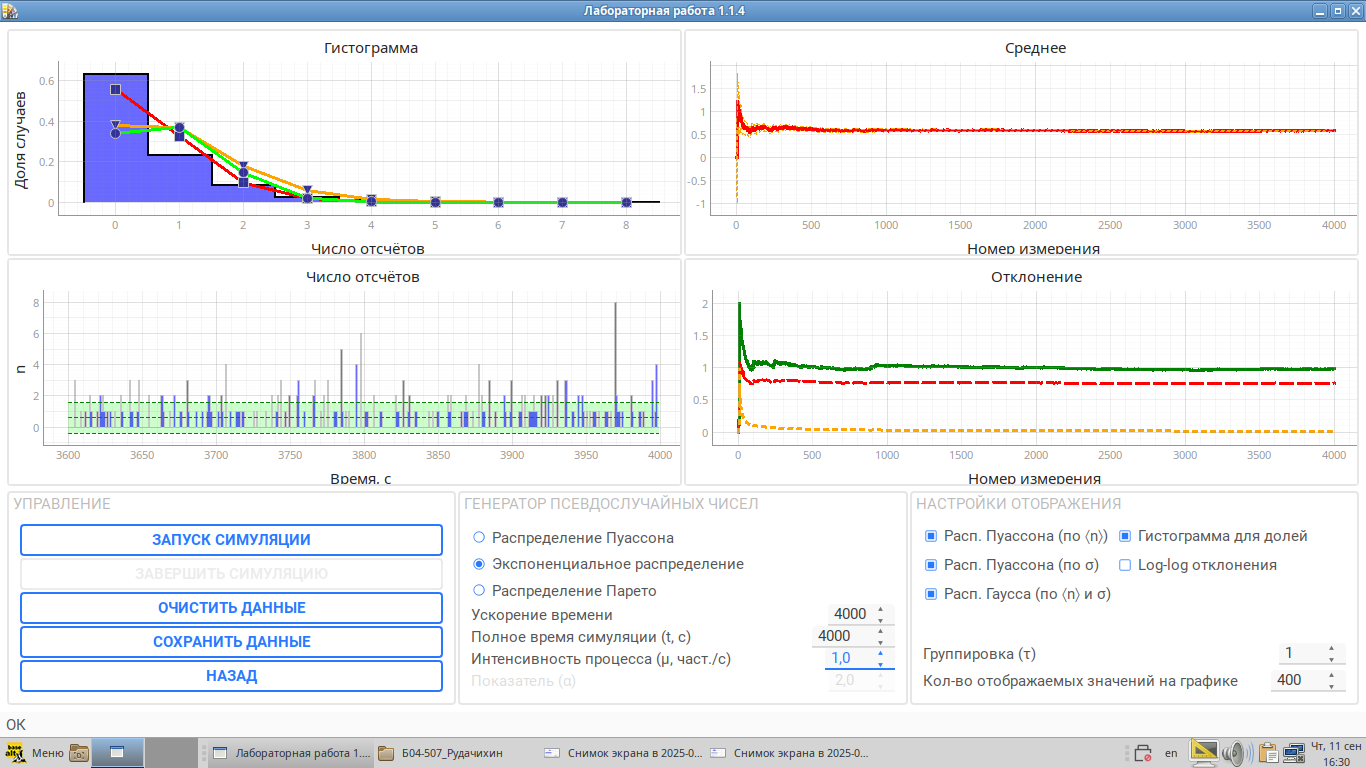
\includegraphics[width=0.9\linewidth]{e1.png} 
			\caption{Средняя интенсивность 1}
			\label{fig:subim31}
		\end{subfigure}
		\begin{subfigure}{0.5\linewidth}
			\centering
			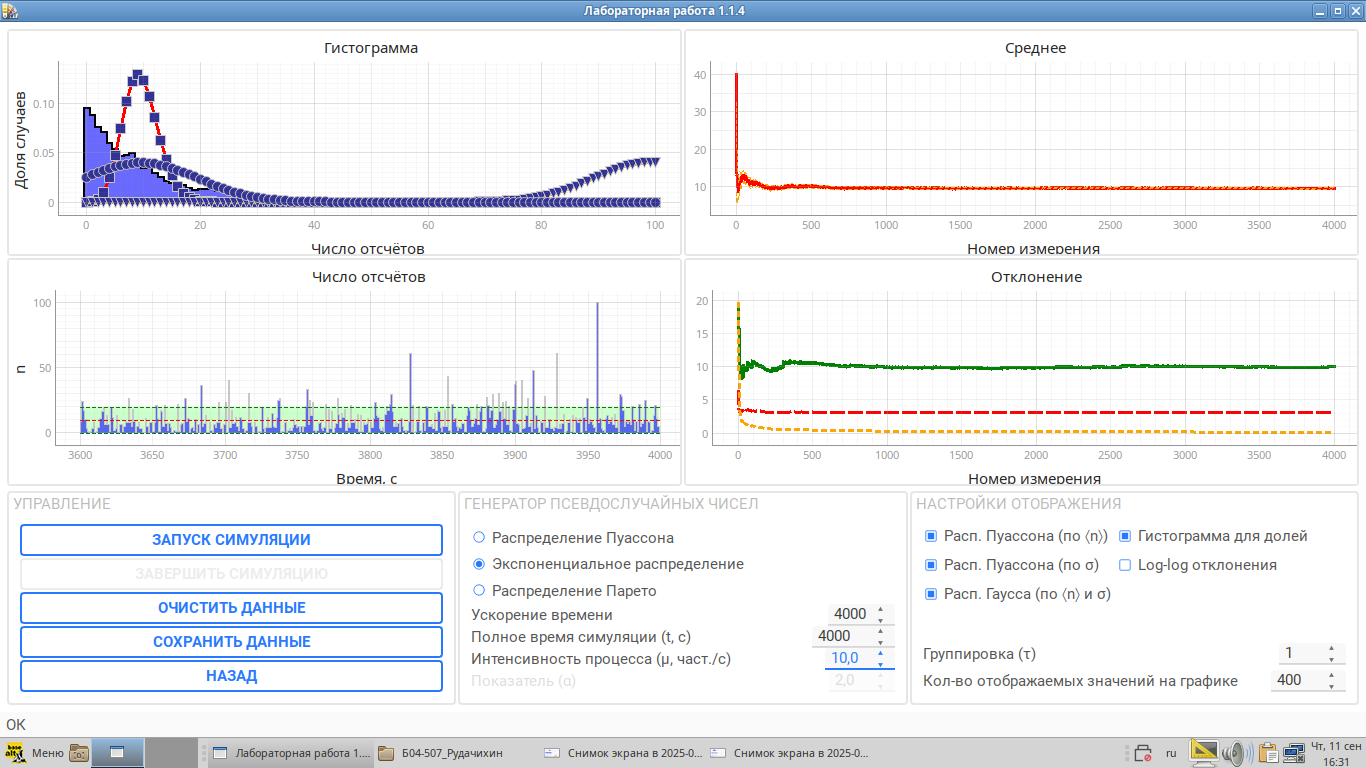
\includegraphics[width=0.9\linewidth]{e10.png}
			\caption{Средняя интенсивность 10}
			\label{fig:subim32}
		\end{subfigure}
		\caption{Симуляция экспоненциального распределения}
		\label{fig:image3}
	\end{figure}
	
	
	
	\begin{figure}[h]
		\begin{subfigure}{0.5\linewidth}
			\centering
			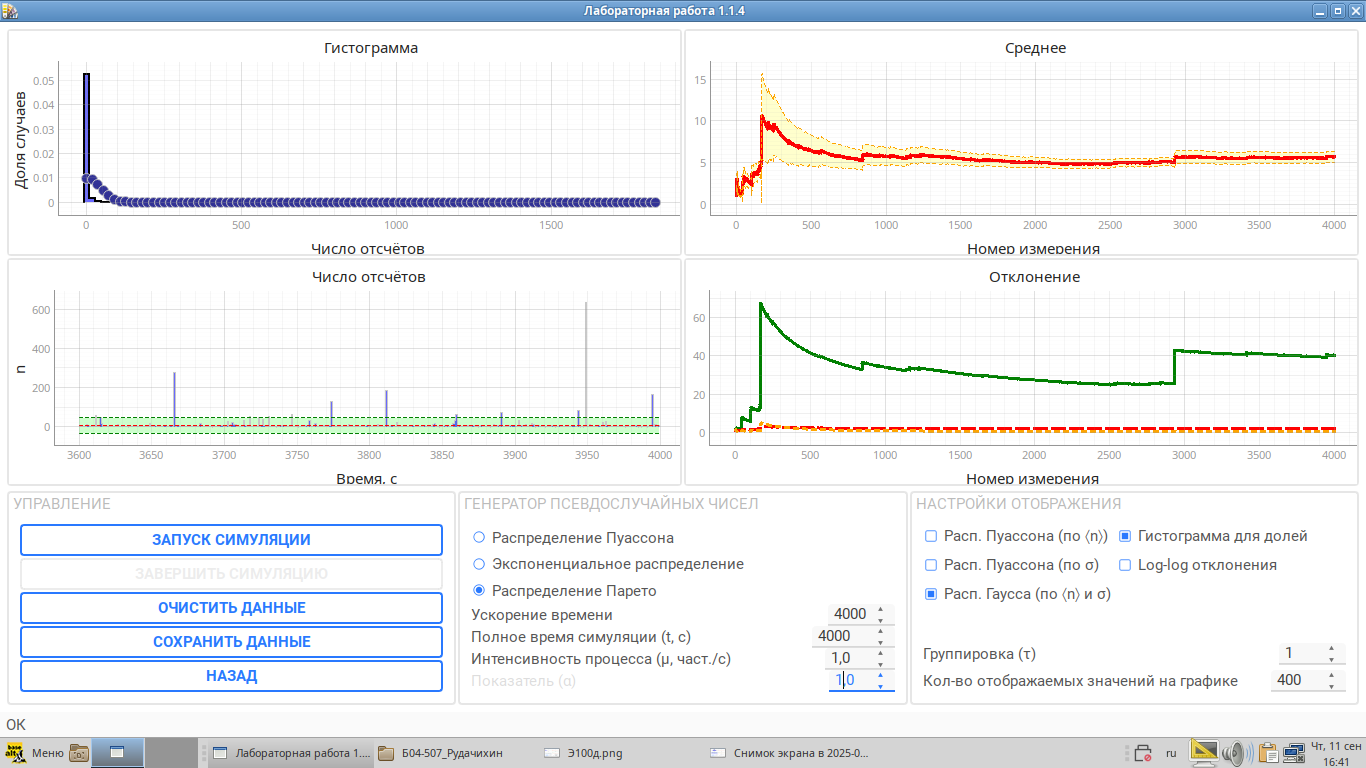
\includegraphics[width=0.9\linewidth]{1p1.png} 
			\caption{Интенсивность = 1, а = 1}
			\label{fig:subim41}
		\end{subfigure}
		\begin{subfigure}{0.5\linewidth}
			\centering
			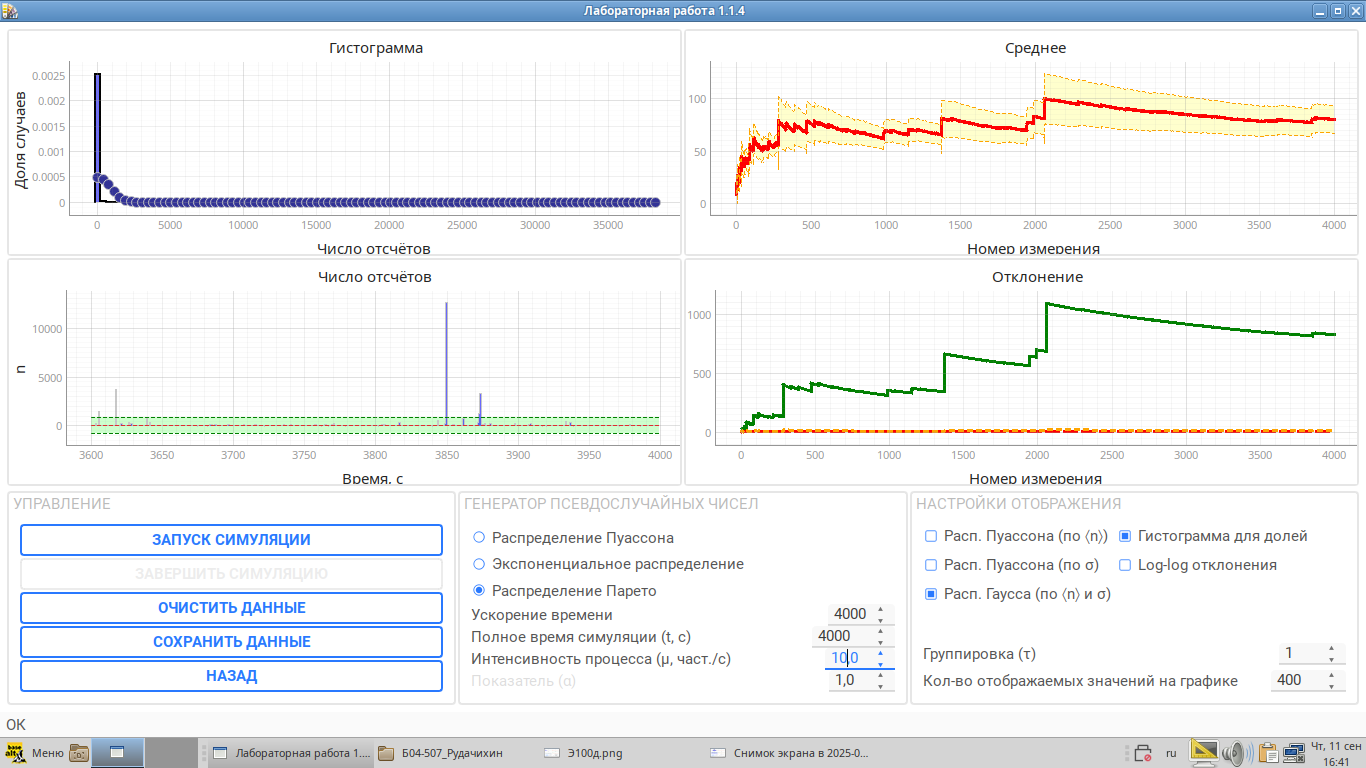
\includegraphics[width=0.9\linewidth]{1p10.png}
			\caption{Интенсивность = 10, а = 1}
			\label{fig:subim42}
		\end{subfigure}
		\begin{subfigure}{0.5\linewidth}
			\centering
			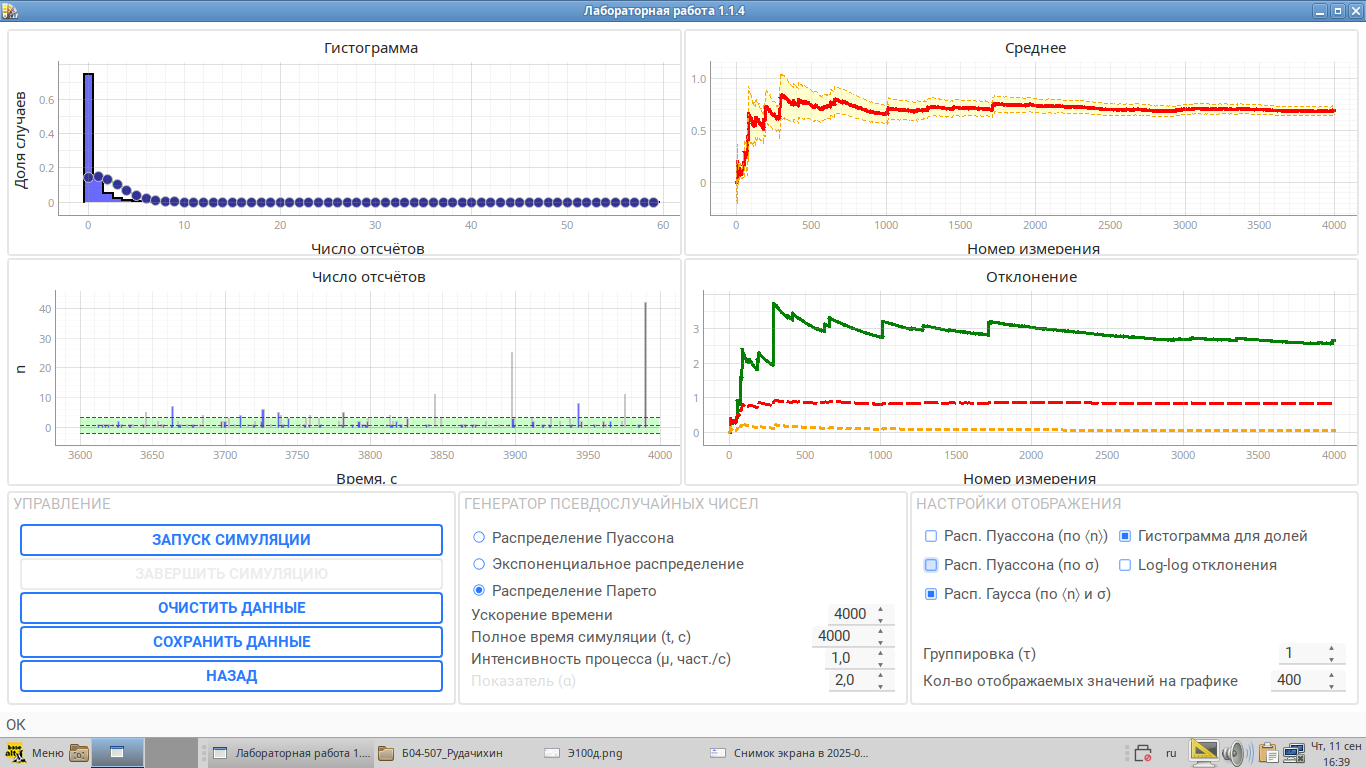
\includegraphics[width=0.9\linewidth]{2p1.png}
			\caption{Интенсивность = 1, а = 2}
			\label{fig:subim43}
		\end{subfigure}
		\begin{subfigure}{0.5\linewidth}
			\centering
			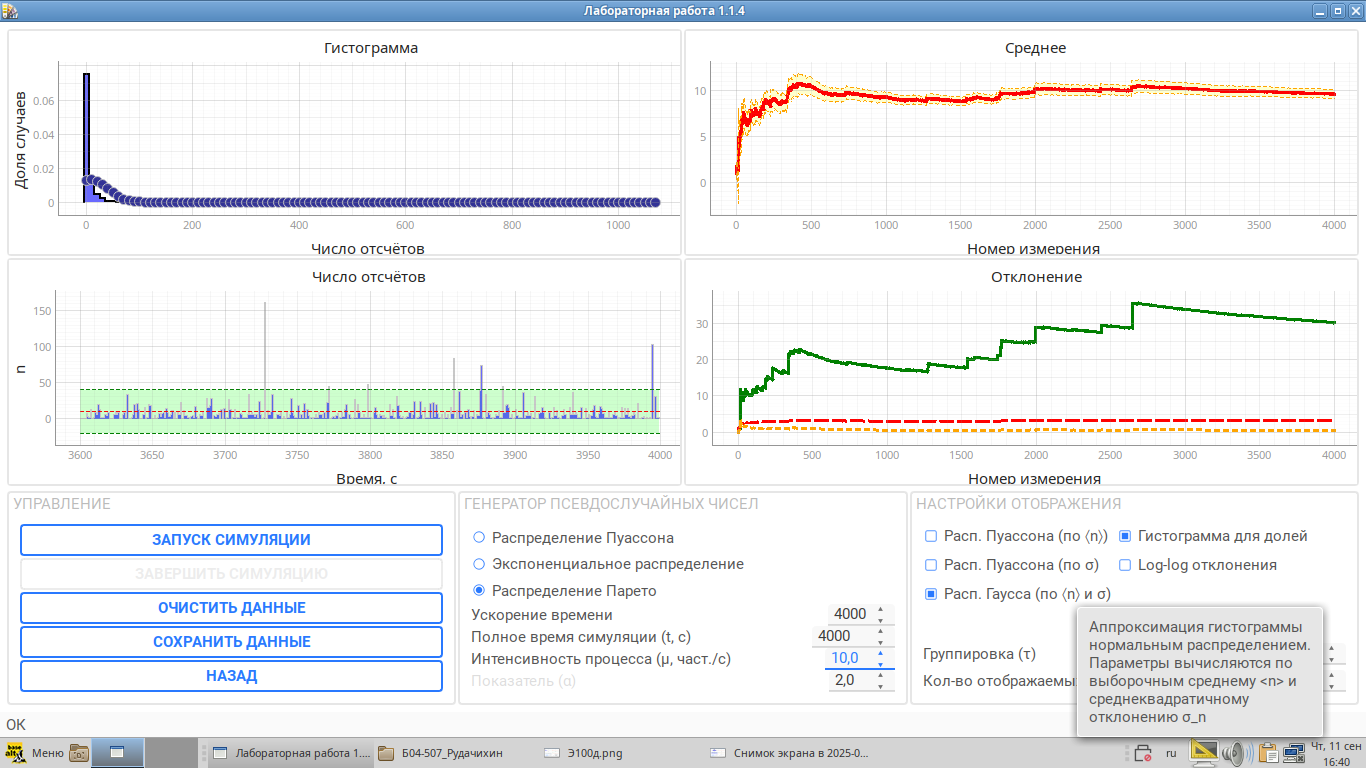
\includegraphics[width=0.9\linewidth]{2p10.png}
			\caption{Интенсивность = 10, а = 1}
			\label{fig:subim44}
		\end{subfigure}
		\caption{Симуляция распределения Парето}
		\label{fig:image4}
	\end{figure}
	
	Полученные в одной из симуляций пуассоновского процесса с единичной средней интенсивностью значения обработаны аналогично демонстрационной программе с помощью языка Python и ПО Microsoft Excel (рис. 9).
	
	\begin{figure}[h!]
		\centering
		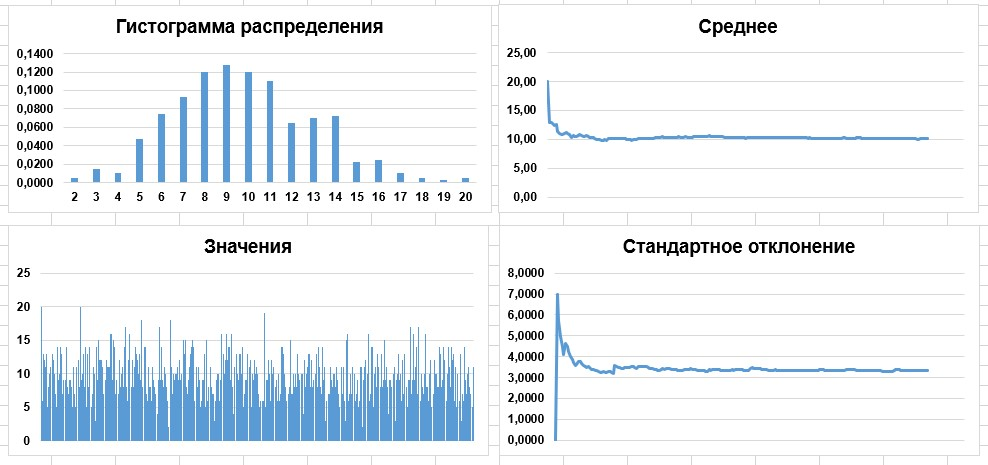
\includegraphics[width=0.8\linewidth]{sim.jpg}
		\caption{Обработка данных одной из симуляций}
		\label{fig:4}
	\end{figure}
	
	\section*{Обработка результатов}
	
	\hspace{4mm} На основе полученных массивов сгруппированных значений вычислены некоторые важные статистические характеристики (табл. 2) и построены гистограммы, на которые наложены графики распределений Пуассона и Гаусса (рис. 10 - 12).
	
	\begin{table}[!h]
		\centering
		\captionbox{Характеристики выборок}{
			\begin{tabular}{|l|rrrr|}
				\hline
				Разбиение & 10 с & 20 с & 40 с & 80 с \\
				\hline
				Среднее  & 10,24    & 20,47    & 40,94    & 81,88 \\
				Стандартное отклонение & 3,32     & 4,73     & 6,44     & 7,93 \\
				Погрешность среднего & 0,17     & 0,33     & 0,64     & 1,12 \\
				Средняя интенсивность & 1,02     & 1,02     & 1,02     & 1,02 \\
				Погрешность интенсивности & 0,02     & 0,02     & 0,02     & 0,02 \\
				Дисперсия & 11,03 &	22,41	& 41,52  & 	62,87 \\
				\hline
				
		\end{tabular}}
		\label{tab:tab1}
	\end{table}%
	
	\begin{figure}[!h]
		\centering
		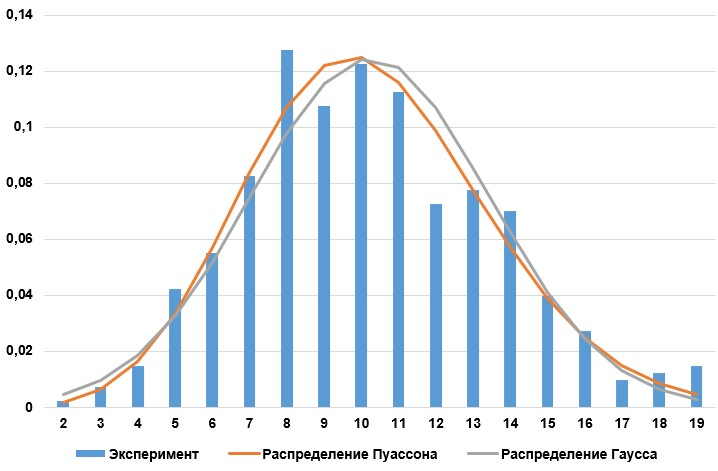
\includegraphics[width=0.7\linewidth]{10.jpg}
		\caption{Интервал разбиения 10 с}
		\label{fig:10}
	\end{figure}
	\begin{figure}[!h]
		\centering
		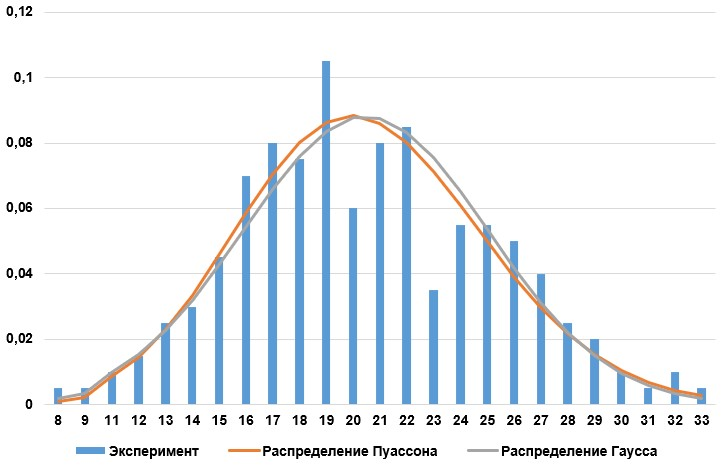
\includegraphics[width=0.7\linewidth]{20.jpg}
		\caption{Интервал разбиения 20 с}
		\label{fig:20}
	\end{figure}
	\begin{figure}[!h]
		\begin{subfigure}{0.5\linewidth}
			\centering
			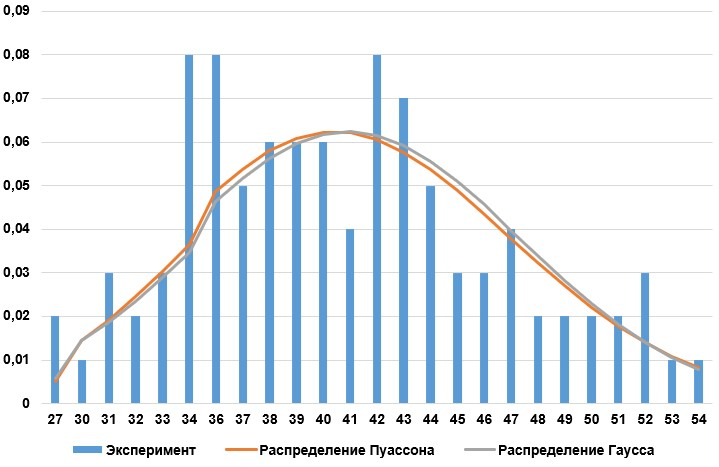
\includegraphics[width=0.95\linewidth]{40.jpg}
			
			\label{fig:40}
		\end{subfigure}
		\begin{subfigure}{0.5\linewidth}
			\centering
			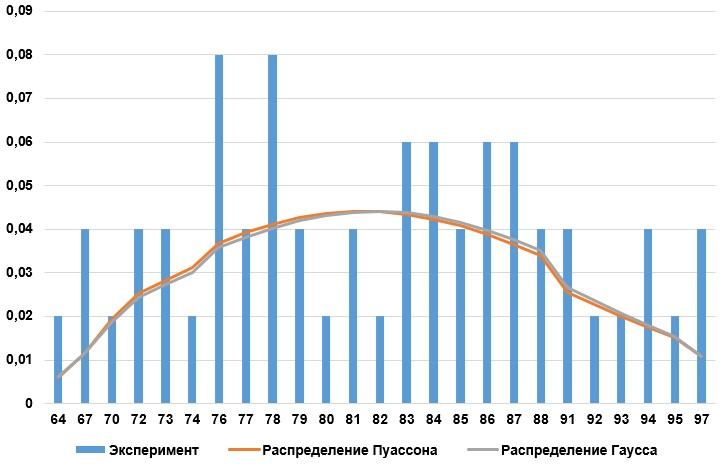
\includegraphics[width=0.95\linewidth]{80.jpg}
			\label{fig:80}
		\end{subfigure}
		\caption{Интервал разбиения 40 с и 80 с}
	\end{figure}
	
	
	
	\section*{Анализ результатов}
		
	\hspace{4mm} Заметим, что лучше всего соотносится с распределениями Пуассона и Гаусса гистограмма для интервала разбиения 10 с. Гистограмма для 20 с тоже соответствует, но её максимум сильно выше максимума теоретических распределений. Гистограммы для интервалов 40 и 80 с совсем не соотносятся с теоретическими графиками, в частности, имеют несколько вершин.
	
	Полученные результаты (табл. 2) прямо зависят от интервала разбиения (чем больше $\tau$, тем больше значения), кроме интенсивности (она постоянна). Заметим, что чем больше количество значений в выборке $N$ (в нашем случае - чем меньше разбиение), тем меньше отклонения и погрешности, что соответствует закону больших чисел.
	
	Значения средних и дисперсий близки (особенно при разбиении 10 с и 40 с), что соответствует свойству распределения Пуассона (7).
	
	Таким образом, распределение частот в полученной выборке соотносится с распределением Пуассона (определено по гистограмме-графику) и выборка с хорошей точностью обладает основным свойством распределения Пуассона (равенство матожидания и дисперсии). Можно заключить, что регистрация космических частиц радиационного фона - реализация пуассоновского процесса.
	
	Проверим выборки на свойство распределения Гаусса, связанное с интервалами значений (табл. 3). Заметим, что полученные доли соответствуют теоретическим значениям. В совокупности с соответствием гистограмм и графиков распределения Гаусса это подтверждает, что полученное для космического излучения распределение близко к нормальному.
	
	\begin{table}[h]
		\centering
		\captionbox{Проверка на свойство распределения Гаусса}{
			\begin{tabular}{|c|c|c|c|c|}
				\hline
				$\tau = $ & 10 c & 20 c & 40 c & 80 c  \\
				\hline
				$\langle x \rangle \pm \sigma$ & 70\% & 70\% & 65\% & 66\%  \\
				\hline
				$\langle x \rangle \pm 2 \sigma$ & 95\% & 95\% & 94\% & 98\%  \\
				\hline
				$\langle x \rangle \pm 3 \sigma$ & 100\% & 100\% & 100\% & 100\%  \\
				\hline
		\end{tabular}}
	\end{table}
	
	
	
	\section*{Заключение}
	\hspace{4mm} Цели работы достигнуты: на примере статистики регистрации фоновых космических частиц изучены статистические закономерности однородного во времени случайного процесса; проверена возможность описания исследуемого процесса статистическими законами Пуассона и Гаусса; измерено среднее число регистрируемых космических лучей в секунду, и определена погрешность результата. 
	
	Подтверждено, что регистрация космического излучения - случайный процесс, с хорошей точностью подчиняющийся законам распределения Пуассона и Гаусса. 
	
	Важным и трудоёмким этапом работы была обработка экспериментальных данных. Основные понятия математической статистики реализованы в характеристиках и графических моделях, которые получены программными средствами Microsoft Excel и языка Python.
	
	
	
	
	
	
\end {document}